\documentclass[a4paper,10pt,fleqn,oneside]{article}
\usepackage{amsmath,amsfonts,amssymb}   %paquetes útiles, contienen símbolos
%\usepackage{enumitem}					%hace más facil manejar listas numeradas
\usepackage[osf,noBBpl]{mathpazo}		%tipo de letra 
\usepackage[utf8]{inputenc}				
\usepackage[T1]{fontenc}				%para poder usar tildes sin problemas
\usepackage[left=1cm,right=1cm,top=1cm,bottom=1cm,headheight=13.6pt]{geometry}
\usepackage{enumerate} % enumerados
\usepackage[utf8]{inputenc} % acentos sin codigo
\usepackage{graphicx}
\usepackage{multicol}

\usepackage[utf8]{inputenc}
\usepackage[spanish]{babel}
\usepackage[poly,arrow,curve,matrix]{xy}
\usepackage{array}
\usepackage{leftidx}
\usepackage{mathrsfs}
\usepackage{graphicx}
\usepackage[ampersand]{easylist}
% Abreviaturas
\newcommand\CC{\mathbb{C}}
\newcommand\RR{\mathbb{R}}
\newcommand\QQ{\mathbb{Q}}
\newcommand\ZZ{\mathbb{Z}}
\newcommand\NN{\mathbb{N}}
\renewcommand\emptyset{\varnothing}
\newcommand\nbd\nobreakdash
\newcommand\Sum{\displaystyle\sum}
\renewcommand{\baselinestretch}{1.2}
\newcommand{\eps}{\varepsilon}
\providecommand{\modu}[1]{\vert\vert#1\vert\vert}
\begin{document}


%%\begin{center}
%%\begin{large}
%Cálculo avanzado - Primer cuatrimestre

%\bigskip
%Ejercicio para entregar

%\bigskip
%Bryan Malpartida
%\end{large}
%\end{center}
\bigskip
\noindent
\centering
Preguntas de Ferromagnetismo para el pelado botón


\begin{enumerate}[1.]
	\item \textbf{Explique los comportamientos ferromagneticos, paramagneticos y diamagneticos.}
		 
		 Los materiales ferromagnéticos son aquellos que adquieren magnetización al ser expuestos a un campo magnético y la mantienen una vez que este es removido. Los paramagnéticos son los que adquieren magnetización al ser expuestos, pero la pierden inmediatamente cuando el campo desaparece, por lo que no tienen memoria. Finalmente, los diamagnéticos son aquellos que adquieren magnetización que tiende a oponerse al campo magnético al que están siendo expuestos, pero también la pierden al desaparecer el campo como un paramagnético.
	\item \textbf{¿Qué es una curva de histéresis? Grafique e indique la magnetización remanente y la coercitividad.}
	
		La curva de histéresis muestra la magnetización de un material en función a la intensidad del campo magnético que la induce. Cabe destacar que un mismo material puede tener varios ciclos de histéresis dependiendo del valor de la excitación máxima y mínimo que se aplique.

\begin{figure}[h]
	\centering
	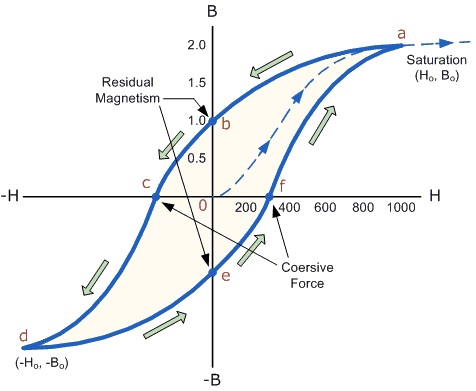
\includegraphics[scale=0.5]{histeresis.jpg}
	\caption{Hola, soy la curva de histéresis}
	\label{CH}
\end{figure}		
		
	\item \textbf{¿Qué es la temperatura de Curie? Explique que sucede con el material por debajo y por encima de la $\mathbf{T_c}$.}
	
	La temperatura de Curie de un material es la temperatura a partir de la cual el material pasa de un comportamiento ferromagnético a paramagnético. Por ensima de la $T_c$, la entropía del material es demasiado alta como para mantener una magnetización remanente. 
	\item \textbf{¿Qué son los materiales magnéticamente duros y blandos?¿Para qué se usan?}
	
	Los materiales magnéticamente duros son aquellos que, una vez magnetizados, conservan dicha magnetización de manera permanente, mientras que los blandos tienden a perderla fácilmente.
	Los duros se pueden utilizar en motores eléctricos y generadores de corriente continua entre otros; y los blandos se pueden usar en transformadores, generadores, electroimanes etc.
	
	\item \textbf{¿Cómo funciona un transformador, un transformador diferencial y un auto-transformador?¿Para qué se usa cada uno?}
	
	\begin{figure}[h]
		\centering
		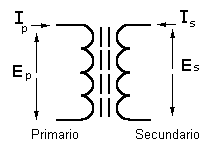
\includegraphics[scale=0.6]{Trans.png}
		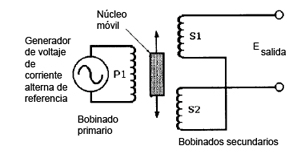
\includegraphics[scale=0.6]{TransDif.jpg}
		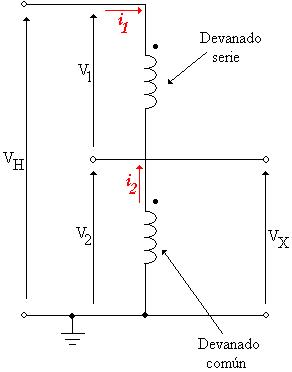
\includegraphics[scale=0.45]{AutoTrans.jpg}
		\caption{Transformador común, diferencial y autotransformador (de izquierda a derecha)}
		\label{CH}
	\end{figure}
	
	Un transformador consiste de dos bobinas acopladas alrededor de un nucleo ferromagnético que modifican la tensión de entrada de forma tal que $E_s N_s = \pm E_pN_p$, dependiendo del sentido relativo de los embobinados. Se usa justamente entre fuente y dispositivo para transformar la tensión de la fuente en la tensión a la que el dispositivo opera.
	
	Un transformador diferencial consiste de 2 bobinas secundarias, una bobina primaria y un núcleo móvil. La bobina primaria induce tensión en las secundarias, las cuales al estar invertidas proporcionan un $E_s$ igual a la resta de sus voltajes. Sin embargo, el núcleo puede moverse, modificando las inductancias y, así, la $E_s$. Dada la sensibilidad de $E_s$ ante movimientos del núcleo, suelen usarse para medir pequeños desplazamientos como en las balanzas electrónicas y otros instrumentos de medición electrónica.
	
	Por último, un autotransformador consiste de una única bobina alrededor de un nucleo ferromagnético con una terminal que sale a una cierta altura del mismo. La relación de voltajes es $V_H=\frac{N_1}{N_1+N_2}V_X$. Estos transformadores se utilizan para interconectar circuitos que funcionan a tensiones diferentes pero con relación aproximadamente 2:1 y para sistemas de distribución eléctrica a grandes distancias dado que con ellos la caída de tensión es menor.
	
	\item \textbf{¿Cómo funciona un circuito integrador? Calcule la función de transferencia y la frecuencia de corte.} 
	
	\begin{figure}[h]
		\centering
		\includegraphics[scale=0.75]{integrador.png}
		\caption{Hola, soy un circuito pedorro}
		\label{Int}
	\end{figure}
	
	El voltaje de salida $complejo$ es \[\mathbb{V}_s = \frac{Z_c}{Z}\mathbb{V}_e = \frac{\mathbb{V}_e}{(R+\frac{1}{i\omega C})i\omega C} = \frac{V_ee^{i\omega t}}{1+i\omega CR}\approx \frac{V_e e^{i\omega t} }{i\omega C R} = \frac{1}{RC}\int \mathbb{V}_e dt\]
	donde usamos que $\omega CR\gg 1$. Bajo esta aproximación vemos que la señal de salida es proporcional a la primitiva de la señal de entrada. Esto es equivalente a $\omega \gg 1/RC \equiv \omega_c$ por lo que tenemos una frecuencia de corte \[ f_c = \frac{1}{2\pi RC} \]
	
	La función de transferencia para este circuito es \[ T(\omega) = \Big| \frac{\mathbb{V}_s}{\mathbb{V}_e} \Big| = \frac{1}{\sqrt{1+\big( \frac{\omega}{\omega_c} \big)^2}}\approx \frac{\omega_c}{\omega} \qquad \text{para } \omega\gg \omega_c \]
	
	\item \textbf{¿Qué significa la integral de la curva de histéresis?}
	
	El área bajo la curva es proporcional a la energía perdida como calor durante la magnetización. 
	\item \textbf{¿Depende el comportamiento de hístéresis de la frecuencia?¿Y de la temperatura? Explique.}
	
\end{enumerate}


\end{document}
